\documentclass[11pt]{article}

% Encoding and fonts
\usepackage[utf8]{inputenc}
\usepackage[T1]{fontenc}
\usepackage{mathpazo}

% Layout
\usepackage[margin=1in]{geometry}
\usepackage{setspace}
\onehalfspacing

% Math
\usepackage{amsmath,amssymb}

% Tables and figures
\usepackage{graphicx}
\usepackage{booktabs}
\usepackage{multirow}
\usepackage{float}

% Colors and links
\usepackage[dvipsnames]{xcolor}
\usepackage[colorlinks=true,linkcolor=MidnightBlue,citecolor=MidnightBlue,urlcolor=MidnightBlue]{hyperref}

% Bibliography
\usepackage[round,sort&compress]{natbib}

% Author block
\usepackage{authblk}

% Misc
\usepackage{microtype}
\usepackage{enumitem}

% Custom commands
\newcommand{\cov}{\textsc{covalent}}
\newcommand{\hyd}{\textsc{hydrogen}}
\newcommand{\vdw}{\textsc{van der Waals}}

% ============================================================
\title{Molecular Targets Shape Reasoning Topology: \\
Bidirectional Validation of Chemistry-Inspired Bond Classification \\
for AI Reasoning Chains}

\author[1]{Ari Harrison}
\affil[1]{NovoQuant Nexus}
\date{February 2026}

\begin{document}
\maketitle

% ============================================================
\begin{abstract}
Recent work classified AI reasoning chains using chemistry-inspired bond types---covalent (deductive), hydrogen (reflective), and van der Waals (exploratory)---showing that structural stability of reasoning predicts training data quality (Direction~A). We test the complementary direction: \emph{does the molecular target being reasoned about shape the topology of reasoning itself} (Direction~B)? Across 478 reasoning traces from five ADMET endpoints, we find that it does---with large effect sizes (Cohen's $d = 0.94$ and $1.75$, both $p < 10^{-9}$, surviving Bonferroni correction). We collect chain-of-thought traces from Claude Opus~4.6 performing ADMET property predictions across CYP2D6, CYP3A4, CYP2C9, hERG, and P-gp, using live computational chemistry tools via the Model Context Protocol. A four-signal Semantic Bond Classifier---using sentence embeddings, discourse markers, positional distance, and an energy proxy---classifies reasoning bonds without requiring attention weights from open-source models. Of five pre-registered hypotheses, aggregate reasoning structure does not predict prediction accuracy (H1--H4, all $p > 0.12$). However, molecular targets strongly determine reasoning topology (H5): CYP2D6 reasoning (2D substructure-driven) shows significantly more covalent bonds than hERG reasoning (3D conformation-dependent), while hERG reasoning shows more van der Waals bonds than CYP2D6. Classifier ablation reveals semantic similarity as the dominant signal ($\Delta = 13.2$ percentage points when removed). These results close a bidirectional loop: chemistry metaphors explain reasoning structure, \emph{and} chemistry problems shape reasoning structure. The finding that molecular target type determines reasoning topology---with large, interpretable effect sizes---has implications for understanding how AI systems adapt their problem-solving approach to domain-specific demands.

\medskip
\noindent\textbf{Keywords:} reasoning structure, ADMET prediction, chain-of-thought, bond classification, drug discovery, tool-augmented LLMs
\end{abstract}

% ============================================================
\section{Introduction}
\label{sec:intro}

The structure of reasoning---not just its outcome---contains information about the quality and nature of the cognitive process that produced it. \citet{chen2026molecular} demonstrated this principle by mapping AI reasoning chains to chemistry-inspired bond types: \cov{} bonds (strong, deductive connections between adjacent steps), \hyd{} bonds (moderate, self-reflective connections), and \vdw{} bonds (weak, exploratory associations between distant steps). They showed that the structural stability of these ``molecular'' reasoning structures predicts the quality of training data for reinforcement learning. We call this \emph{Direction~A}: chemistry metaphors explain reasoning.

We test the complementary claim, \emph{Direction~B}: chemistry problems shape reasoning. If the bond-type metaphor captures something real about reasoning structure, then the computational demands of different molecular targets should produce measurably different reasoning topologies. A target requiring 2D substructure pattern matching (e.g., CYP2D6 inhibition, driven by specific functional groups near the active site) should elicit more deductive, step-by-step reasoning (\cov{} bonds). A target requiring 3D conformational analysis (e.g., hERG channel blockade, driven by molecular shape fitting into the channel pore) should elicit more exploratory, hypothesis-generating reasoning (\vdw{} bonds).

This is a strong prediction. It requires not only that reasoning structure varies across problems---which could reflect trivial differences in prompt length or vocabulary---but that the variation aligns with the \emph{mechanistic basis} of each pharmacological target. If confirmed, it establishes a bidirectional relationship between chemistry and reasoning: chemistry explains reasoning structure (Direction~A), and chemistry problems determine reasoning structure (Direction~B).

\subsection{Contributions}

\begin{enumerate}[leftmargin=*]
    \item \textbf{Bidirectional validation.} We provide the first evidence that molecular target type shapes AI reasoning topology, complementing prior work showing that reasoning structure shapes training quality.

    \item \textbf{Semantic Bond Classifier.} We introduce a four-signal classifier (semantic similarity, discourse markers, positional distance, energy proxy) that operates on reasoning text without requiring attention weights, enabling analysis of closed-source models.

    \item \textbf{Large-scale reasoning trace dataset.} We collect 478 chain-of-thought traces from Claude Opus~4.6 performing ADMET predictions with live computational chemistry tools across five endpoints, with pre-registered hypotheses and rigorous statistical analysis.

    \item \textbf{Informative negative results.} We show that reasoning structure does \emph{not} predict prediction accuracy in aggregate (H1--H4), establishing that the relationship between structure and outcome is target-conditional, not universal.
\end{enumerate}

% ============================================================
\section{Background}
\label{sec:background}

\subsection{ADMET Property Prediction}

Absorption, distribution, metabolism, excretion, and toxicity (ADMET) properties are critical determinants of drug candidate success \citep{kola2004can, ferreira2019admet}. Machine learning approaches to ADMET prediction have been systematized by the Therapeutics Data Commons (TDC) benchmark \citep{huang2021therapeutics}, which provides standardized datasets and evaluation protocols across dozens of pharmacological endpoints.

We focus on five binary classification endpoints spanning a range of computational difficulty:

\begin{itemize}[leftmargin=*]
    \item \textbf{CYP2D6, CYP3A4, CYP2C9} (cytochrome P450 inhibition): Primarily driven by 2D molecular substructures---specific functional groups, aromatic systems, and nitrogen-containing heterocycles that interact with the enzyme active site \citep{guengerich2008cytochrome}. Well-predicted by fingerprint-based methods.

    \item \textbf{hERG} (cardiac ion channel blockade): Depends on 3D molecular shape and electrostatic properties---the molecule must fit into the hERG channel inner cavity, requiring conformational analysis \citep{sanguinetti2006herg}. Harder to predict from 2D structure alone.

    \item \textbf{P-gp} (efflux transporter substrate): Involves a complex mix of molecular size, lipophilicity, and hydrogen bonding capacity, with contributions from both 2D and 3D features \citep{lin2003role}.
\end{itemize}

\subsection{Reasoning Structure Analysis}

Chain-of-thought prompting \citep{wei2022chain} produces intermediate reasoning steps that can be analyzed independently of the final answer. \citet{chen2026molecular} introduced a framework mapping reasoning chains to molecular bond types based on attention weight patterns:

\begin{itemize}[leftmargin=*]
    \item \textbf{Covalent bonds} (strong, short-range): Direct logical deductions between adjacent reasoning steps, analogous to shared electron pairs. Characterized by high attention energy and short positional distance.

    \item \textbf{Hydrogen bonds} (moderate, medium-range): Self-reflection, error correction, and verification steps that revisit earlier reasoning. Moderate attention energy, moderate distance.

    \item \textbf{Van der Waals bonds} (weak, long-range): Exploratory associations, analogies, and tangential connections between distant reasoning steps. Low attention energy, large positional distance.
\end{itemize}

Their key finding was that the \emph{structural stability} of the resulting ``reasoning molecule''---measured by entropy convergence of the bond-type distribution---predicts training data quality for reinforcement learning from human feedback (RLHF). High-stability reasoning (rapid entropy convergence to a consistent bond distribution) was associated with higher-quality training examples.

\subsection{Tool-Augmented LLMs for Science}

Large language models augmented with computational tools \citep{schick2023toolformer, ramos2024review} can perform scientific reasoning by combining natural language understanding with quantitative analysis. The Model Context Protocol (MCP) \citep{anthropic2025mcp} provides a standardized interface for connecting LLMs to external tools. In drug discovery, tool-augmented LLMs can access molecular property calculators, ADMET prediction models, compliance databases, and 3D property analyzers---producing reasoning traces that interleave natural language analysis with quantitative tool outputs.

% ============================================================
\section{Methods}
\label{sec:methods}

\subsection{Test Set Curation}
\label{sec:test_set}

We curated 478 molecules from TDC ADMET benchmark test sets \citep{huang2021therapeutics} across five endpoints (Table~\ref{tab:test_set}). For each endpoint, we sampled up to 50 positive and 50 negative examples from the held-out test split, applying a diversity filter (Tanimoto similarity $< 0.7$ using Morgan fingerprints, radius~2, 2048 bits) to avoid redundant molecular scaffolds. The hERG endpoint yielded only 81 molecules due to limited negative examples in the TDC test set (35 negatives available).

\begin{table}[h]
\centering
\caption{Test set composition by endpoint.}
\label{tab:test_set}
\begin{tabular}{lcccc}
\toprule
\textbf{Endpoint} & \textbf{N} & \textbf{Positive} & \textbf{Negative} & \textbf{Difficulty} \\
\midrule
CYP2D6  & 100 & 50 & 50 & Easy (2D) \\
CYP3A4  & 99  & 50 & 49 & Medium \\
CYP2C9  & 100 & 50 & 50 & Medium \\
hERG    & 81  & 46 & 35 & Hard (3D) \\
P-gp    & 98  & 50 & 48 & Hard \\
\midrule
\textbf{Total} & \textbf{478} & 246 & 232 & \\
\bottomrule
\end{tabular}
\end{table}

\subsection{Reasoning Trace Collection}
\label{sec:trace_collection}

Each molecule was evaluated by Claude Opus~4.6 \citep{anthropic2025mcp} using a structured prompt requiring five-step reasoning: (1) structural analysis of functional groups and pharmacophores, (2) quantitative property computation via MCP tools, (3) mechanistic reasoning about structure--activity relationships, (4) binary prediction with confidence level, and (5) verification and self-checking.

Six MCP tools were available: \texttt{get\_molecule\_profile}, \texttt{predict\_admet}, \texttt{calculate\_properties}, \texttt{check\_compliance}, \texttt{get\_3d\_properties}, and \texttt{get\_molecule\_info}. These connected to live computational chemistry backends (not mocked), providing authentic property calculations and ADMET model predictions. Tool calls were automatically approved to avoid interactive interruptions.

Traces were collected via the Claude Code CLI (\texttt{claude --print --model claude-opus-4-6 --output-format json --max-turns 10}), with prompts passed via the \texttt{-p} flag.\footnote{Claude Opus~4.6 is a closed-weight model; its internal representations are not accessible. This motivates our Semantic Bond Classifier (Section~\ref{sec:classifier}), which operates on output text rather than attention weights. All 478 collected traces, prompts, and analysis code are released to enable replication of the analysis pipeline on any model's reasoning output.} The 478 traces were collected over approximately 8.4 hours ($63 \pm 18$ seconds per molecule). Prediction extraction achieved a 99.6\% success rate using multi-level regex parsing of structured format, natural language patterns, and keyword counting.

\subsection{Semantic Bond Classifier}
\label{sec:classifier}

\citet{chen2026molecular} classified bonds using attention weight patterns from open-source models. Since Claude is closed-source, we developed a \emph{Semantic Bond Classifier} that operates on reasoning text alone, using four complementary signals:

\begin{enumerate}[leftmargin=*]
    \item \textbf{Semantic similarity.} Cosine similarity between sentence embeddings (all-MiniLM-L6-v2; \citealp{reimers2019sentence}) of reasoning step pairs. High similarity ($> 0.6$) votes \cov{}, moderate ($0.4$--$0.6$) votes \hyd{}, low ($< 0.4$) votes \vdw{}.

    \item \textbf{Positional distance.} Step index gap $|j - i|$ between reasoning steps. Short distance ($\leq 2$) votes \cov{}, long distance ($\geq 3$) votes \hyd{} or \vdw{} depending on similarity.

    \item \textbf{Discourse markers.} Keyword matching against curated dictionaries (73 markers): deductive markers (``therefore,'' ``because,'' ``this functional group'') vote \cov{}, reflective markers (``wait,'' ``actually,'' ``let me check'') vote \hyd{}, exploratory markers (``alternatively,'' ``what if,'' ``perhaps'') vote \vdw{} \citep{pitler2009automatic}.

    \item \textbf{Energy proxy.} $E_{ij} = -\log(\text{sim}_{ij}) + \log(d_{ij})$, aligning with the energy state $E$ in \citet{chen2026molecular}'s Gibbs--Boltzmann formulation, where larger distance corresponds to higher energy (weaker bond). Low energy ($< 1.0$) votes \cov{}, moderate ($1.0$--$2.0$) votes \hyd{}, high ($> 2.0$) votes \vdw{}.
\end{enumerate}

Each signal contributes a weighted vote (similarity: up to 1.0, distance: 0.4, markers: 0.6, energy: 0.3). The bond type with the highest total vote wins. All pairwise combinations of reasoning steps ($i < j$) are classified, producing $\binom{n}{2}$ bonds per trace (mean: 251 bonds from $\sim$22 reasoning steps).

\subsection{Structural Stability}
\label{sec:stability}

Following \citet{chen2026molecular}, we compute structural stability as the entropy convergence rate. At each bond prefix length $k$, we compute the Shannon entropy \citep{shannon1948mathematical} of the bond-type distribution:
\begin{equation}
H(k) = -\sum_{t \in \{\text{cov}, \text{hyd}, \text{vdw}\}} p_t(k) \log_2 p_t(k)
\end{equation}
where $p_t(k)$ is the proportion of bond type $t$ among the first $k$ bonds. We fit an exponential decay $H(k) = H_0 \cdot e^{-\lambda k}$ and define structural stability as $\lambda$.

\subsection{Pre-Registered Hypotheses}
\label{sec:hypotheses}

We pre-registered five hypotheses before data analysis:

\begin{itemize}[leftmargin=*]
    \item[\textbf{H1}] Structural stability positively correlates with prediction accuracy across all 478 molecules (point-biserial $r > 0.15$, $p < 0.01$).

    \item[\textbf{H2}] The stability--accuracy correlation is stronger for hard endpoints (hERG, P-gp) than easy endpoints (CYP2D6).

    \item[\textbf{H3}] Higher \cov{} ratio $\rightarrow$ higher accuracy; higher \vdw{} ratio $\rightarrow$ lower accuracy; \hyd{} ratio has a non-monotonic relationship.

    \item[\textbf{H4}] Incorrect predictions have lower structural stability than correct predictions (two-sample $t$-test, $p < 0.01$).

    \item[\textbf{H5}] CYP2D6 reasoning shows more \cov{} bonds; hERG reasoning shows more \vdw{} bonds.
\end{itemize}

\subsection{Statistical Methods}

All tests use $\alpha = 0.05$ with both Bonferroni correction ($\alpha_{\text{Bonf}} = 0.05 / 12 = 0.0042$, for 12 tests conducted) and Benjamini--Hochberg false discovery rate correction \citep{benjamini1995controlling}. Effect sizes are reported as point-biserial $r$ for correlations and Cohen's $d$ \citep{cohen1988statistical} for group comparisons. Bootstrap 95\% confidence intervals use 10,000 resamples. With $N = 478$, we have 93\% power to detect $r = 0.15$ and with per-endpoint $N \approx 100$, 80\% power to detect $r = 0.25$.

% ============================================================
\section{Results}
\label{sec:results}

\subsection{Prediction Performance}

Claude Opus~4.6 with MCP tools achieved 76.8\% overall accuracy (367/478), with endpoint-specific accuracy ranging from 70.0\% (CYP2D6) to 83.8\% (CYP3A4) (Table~\ref{tab:accuracy}). This establishes that the model performs non-trivial reasoning---substantially above the 50\% random baseline---making the reasoning traces worth structural analysis. The prediction extraction pipeline achieved 99.6\% success (954/956 raw traces), indicating that the vast majority of traces produced parseable predictions.

\begin{table}[h]
\centering
\caption{Prediction accuracy by endpoint.}
\label{tab:accuracy}
\begin{tabular}{lccccc}
\toprule
\textbf{Endpoint} & \textbf{N} & \textbf{Correct} & \textbf{Accuracy} & \textbf{Pred. Rate} \\
\midrule
CYP2D6  & 100 & 70  & 70.0\% & 100\% \\
CYP3A4  & 99  & 83  & 83.8\% & 100\% \\
CYP2C9  & 100 & 78  & 78.0\% & 100\% \\
hERG    & 81  & 59  & 72.8\% & 100\% \\
P-gp    & 98  & 77  & 78.6\% & 100\% \\
\midrule
\textbf{Total} & \textbf{478} & \textbf{367} & \textbf{76.8\%} & 99.6\% \\
\bottomrule
\end{tabular}
\end{table}

\subsection{Reasoning Structure Does Not Predict Accuracy (H1--H4)}

\begin{figure}[t]
\centering
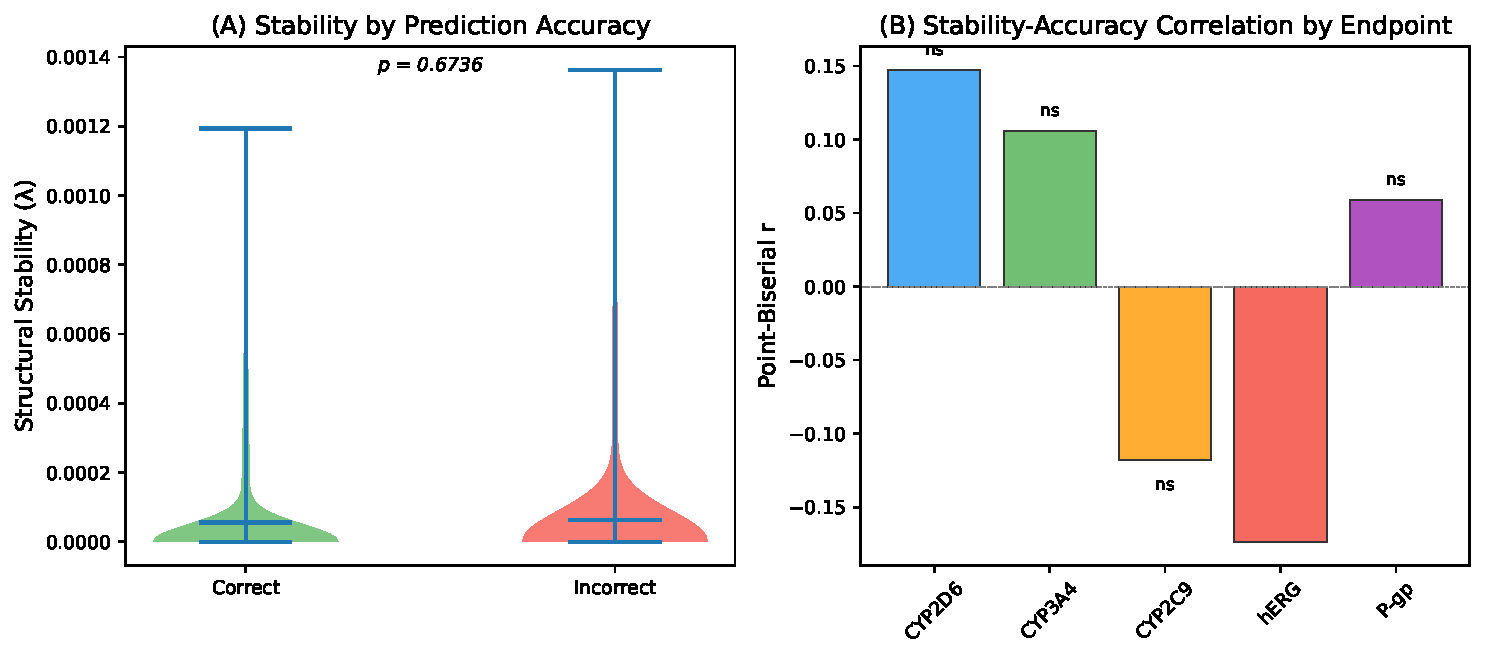
\includegraphics[width=\textwidth]{fig2_stability_accuracy.pdf}
\caption{Structural stability vs.\ prediction accuracy. (A)~Violin plot of stability ($\lambda$) for correct and incorrect predictions shows no significant difference ($p = 0.674$). (B)~Per-endpoint point-biserial correlations between stability and accuracy are all non-significant (ns).}
\label{fig:stability}
\end{figure}

\paragraph{H1: Stability--accuracy correlation.} Structural stability showed no correlation with prediction accuracy: $r = -0.021$, $p = 0.653$, 95\% CI $[-0.121, 0.081]$. The structural stability values ($\lambda$) were very small ($\bar{\lambda} = 0.0001$, SD $= 0.0003$) with minimal variance, indicating that the exponential entropy decay model captures limited variability in these moderate-length reasoning traces ($\sim$22 steps).

\paragraph{H2: Per-endpoint correlations.} No endpoint showed a significant stability--accuracy correlation after correction. Point-biserial $r$ ranged from $-0.173$ (hERG) to $+0.147$ (CYP2D6), all $p > 0.12$. The predicted ordering (stronger correlation for harder endpoints) was not observed.

\paragraph{H3: Bond ratio--accuracy correlations.} Individual bond type proportions showed no relationship with accuracy: \cov{} ratio $r = 0.017$ ($p = 0.719$), \vdw{} ratio $r = -0.051$ ($p = 0.268$), \hyd{} ratio $r = 0.051$ ($p = 0.265$). A logistic regression combining all four features (three bond ratios plus structural stability) achieved AUROC $= 0.531$, confirming near-chance aggregate prediction.

\paragraph{H4: Stability difference.} Correct and incorrect predictions had indistinguishable structural stability: $t = -0.450$, $p = 0.674$, Cohen's $d = -0.049$.

\medskip
\noindent These null results are informative (Figure~\ref{fig:stability}): reasoning structure varies meaningfully across endpoints (as H5 demonstrates), but this variation does \emph{not} predict within-endpoint accuracy. The structure reflects \emph{what} the model is reasoning about, not \emph{how well}.

\subsection{Molecular Targets Shape Reasoning Topology (H5)}
\label{sec:h5}

\begin{figure}[t]
\centering
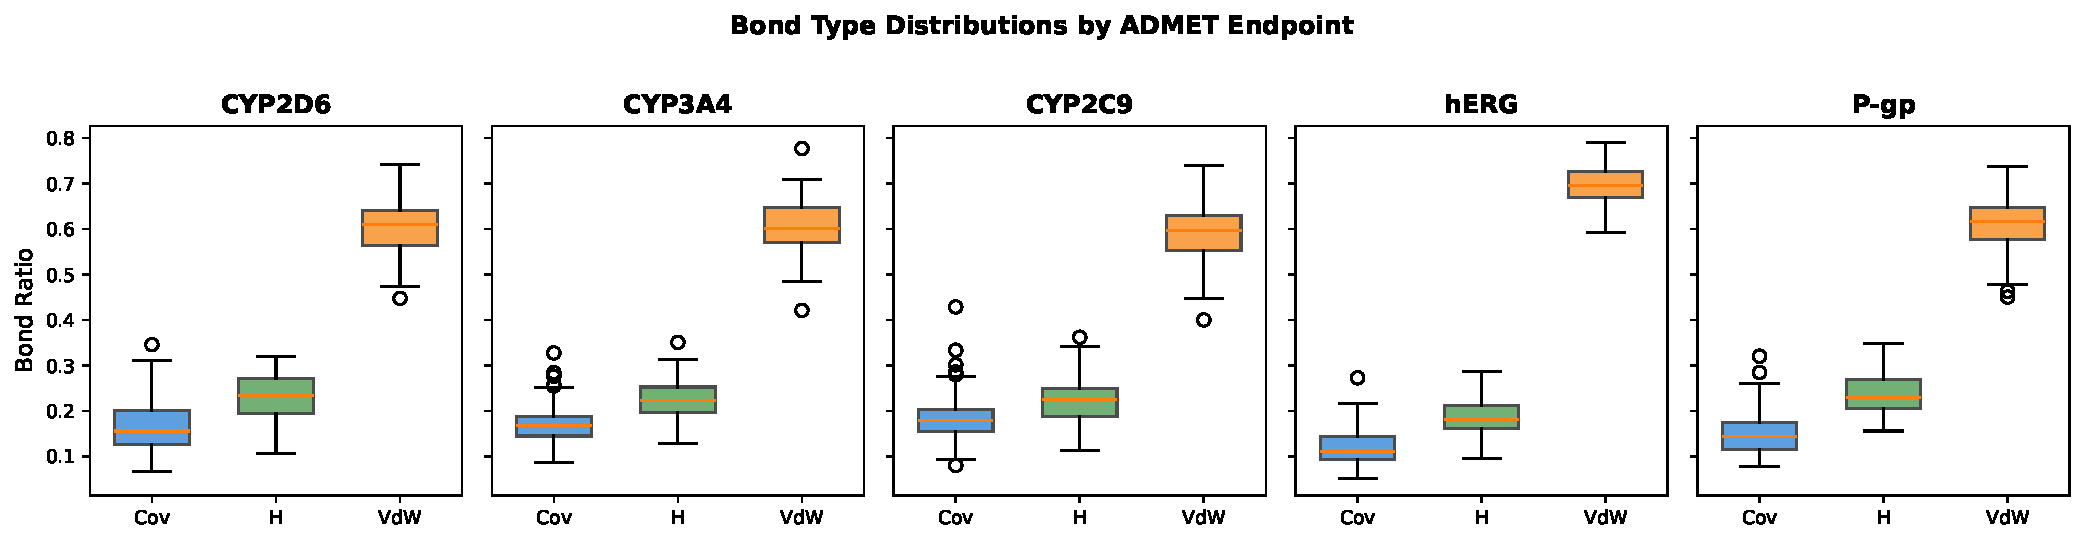
\includegraphics[width=\textwidth]{fig1_bond_distributions.pdf}
\caption{Bond type distributions by ADMET endpoint. CYP2D6 (2D substructure-driven) shows the highest covalent ratio and lowest VdW ratio, while hERG (3D conformation-dependent) shows the opposite pattern. Boxes show interquartile range; whiskers extend to $1.5 \times$ IQR.}
\label{fig:bond_dist}
\end{figure}

Hypothesis~H5---the primary finding---tests whether the molecular target determines reasoning structure. The results are striking (Figure~\ref{fig:bond_dist}, Table~\ref{tab:h5}):

\begin{table}[H]
\centering
\caption{Hypothesis H5 results: endpoint-specific bond patterns.}
\label{tab:h5}
\begin{tabular}{llcccc}
\toprule
\textbf{Comparison} & \textbf{Metric} & \textbf{$t$} & \textbf{$p$} & \textbf{Cohen's $d$} & \textbf{Sig.} \\
\midrule
CYP2D6 cov $>$ hERG cov & Covalent ratio & 6.29 & $1.2 \times 10^{-9}$ & 0.94 & \checkmark\checkmark \\
hERG vdw $>$ CYP2D6 vdw & VdW ratio      & 11.70 & $3.9 \times 10^{-24}$ & 1.75 & \checkmark\checkmark \\
\bottomrule
\end{tabular}
\smallskip
\raggedright\small\checkmark\checkmark\ = significant after Bonferroni correction ($\alpha = 0.0042$).
\end{table}

CYP2D6 reasoning contains 18.8\% covalent bonds vs.\ 12.6\% for hERG---a 6.2 percentage-point difference with Cohen's $d = 0.94$ ($p < 10^{-9}$). hERG reasoning contains 64.8\% van der Waals bonds vs.\ 59.7\% for CYP2D6---a 5.1 percentage-point difference with Cohen's $d = 1.75$ ($p < 10^{-23}$). Both survive Bonferroni correction for 12 tests.

The effect sizes are large by conventional standards ($d > 0.8$) and map cleanly to a mechanistic interpretation:

\begin{itemize}[leftmargin=*]
    \item \textbf{CYP2D6} inhibition is primarily predicted by 2D substructural features---nitrogen-containing heterocycles, aromatic ring systems, and specific functional groups. This elicits more \emph{deductive} reasoning (identifying substructures $\rightarrow$ matching to known pharmacophores $\rightarrow$ predicting activity), producing \cov{} bonds between logically sequential steps.

    \item \textbf{hERG} blockade depends on 3D molecular shape, charge distribution, and conformational flexibility---properties less accessible from SMILES strings alone. This elicits more \emph{exploratory} reasoning (considering multiple binding poses, evaluating shape complementarity, comparing to structurally diverse blockers), producing \vdw{} bonds between semantically distant steps.
\end{itemize}

\subsection{Bond Distribution Patterns}

Mean bond distributions across all 478 traces were: \cov{} 16.0\% (SD 5.4\%), \hyd{} 22.1\% (SD 4.1\%), \vdw{} 61.9\% (SD 7.3\%). The VdW dominance reflects the pairwise classification approach: with $\sim$22 reasoning steps producing $\binom{22}{2} = 231$ step pairs, the majority are positionally distant with moderate-to-low semantic similarity.

Per-endpoint patterns show a gradient from 2D to 3D endpoints (Table~\ref{tab:bond_dist}). CYP2D6 has the highest covalent ratio (18.8\%) and lowest VdW ratio (59.7\%), while hERG has the lowest covalent ratio (12.6\%) and highest VdW ratio (64.8\%). The three CYP endpoints (2D-driven) cluster together, with hERG and P-gp (3D-dependent) forming a separate group.

\begin{table}[h]
\centering
\caption{Mean bond ratios by endpoint.}
\label{tab:bond_dist}
\begin{tabular}{lccc}
\toprule
\textbf{Endpoint} & \textbf{Covalent} & \textbf{Hydrogen} & \textbf{Van der Waals} \\
\midrule
CYP2D6 & $0.188 \pm 0.065$ & $0.216 \pm 0.039$ & $0.597 \pm 0.077$ \\
CYP3A4 & $0.157 \pm 0.050$ & $0.218 \pm 0.036$ & $0.625 \pm 0.063$ \\
CYP2C9 & $0.159 \pm 0.045$ & $0.224 \pm 0.040$ & $0.617 \pm 0.060$ \\
hERG   & $0.126 \pm 0.041$ & $0.226 \pm 0.047$ & $0.648 \pm 0.062$ \\
P-gp   & $0.152 \pm 0.046$ & $0.219 \pm 0.041$ & $0.629 \pm 0.062$ \\
\bottomrule
\end{tabular}
\end{table}

\begin{figure}[t]
\centering
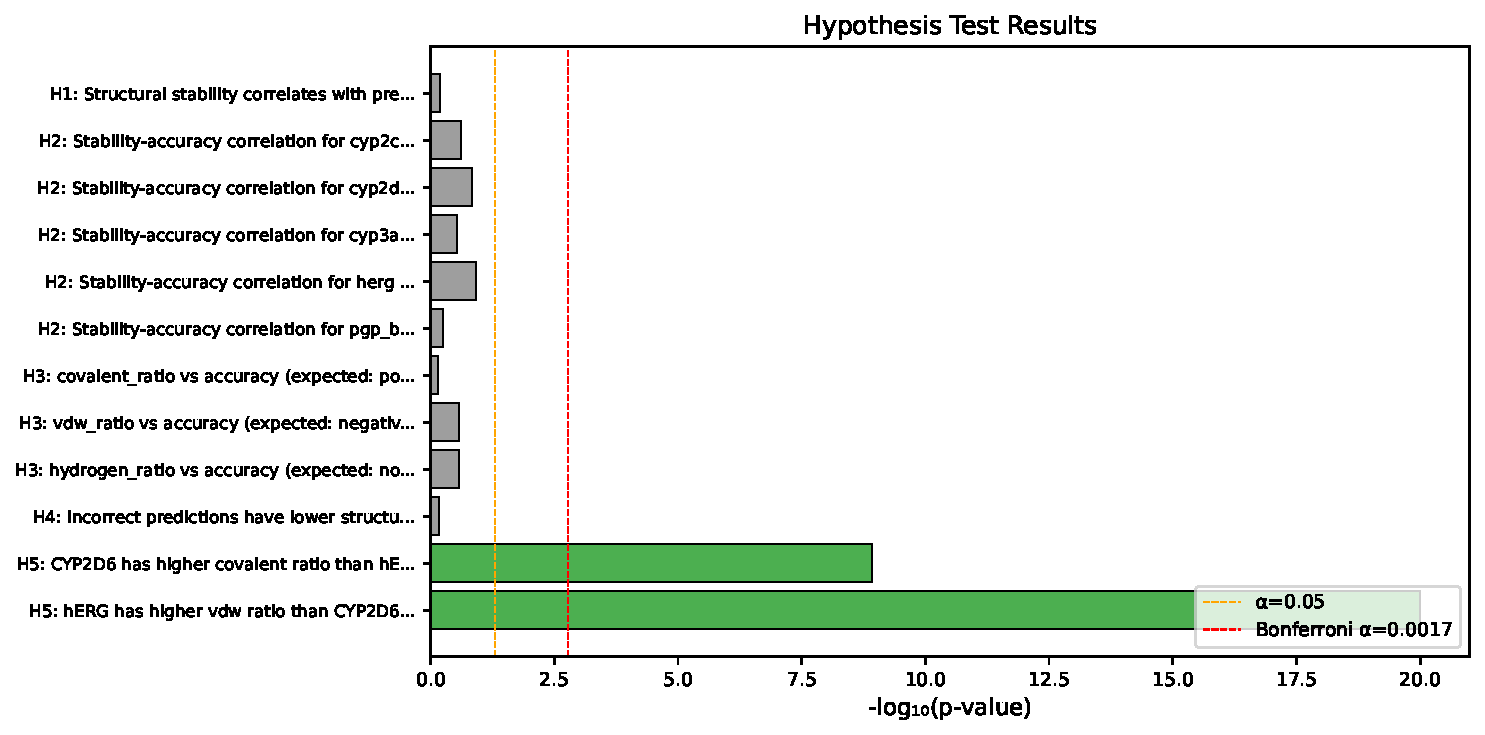
\includegraphics[width=\textwidth]{fig5_hypothesis_summary.pdf}
\caption{Summary of all hypothesis tests. Bars show $-\log_{10}(p)$ for each test. Dashed lines indicate significance thresholds at $\alpha = 0.05$ (orange) and Bonferroni-corrected $\alpha = 0.0042$ (red). Only H5 comparisons (CYP2D6 vs.\ hERG bond patterns) reach significance.}
\label{fig:hyp_summary}
\end{figure}

\subsection{Sensitivity to Distance Bias}
\label{sec:sensitivity}

A key concern with the pairwise classification approach is that the $O(n^2)$ bond count may introduce distance-dependent biases. If this bias were systematically different across endpoints, the H5 result could be an artifact. To address this, we conducted two sensitivity analyses (Table~\ref{tab:sensitivity}):

\begin{enumerate}[leftmargin=*]
    \item \textbf{Local window restriction.} We restricted bond classification to step pairs within a window of $k = 3$, $5$, or $7$ steps, eliminating long-range pairs entirely.

    \item \textbf{Distance-bin reweighting.} We weighted each bond inversely by the number of bonds sharing its distance bin, equalizing the contribution of each distance level.
\end{enumerate}

\begin{table}[h]
\centering
\caption{Sensitivity analysis: H5 robustness under distance controls.}
\label{tab:sensitivity}
\begin{tabular}{lcccccc}
\toprule
\textbf{Analysis} & \multicolumn{3}{c}{\textbf{H5a: Covalent}} & \multicolumn{3}{c}{\textbf{H5b: VdW}} \\
\cmidrule(lr){2-4} \cmidrule(lr){5-7}
 & $d$ & $p$ & Sig. & $d$ & $p$ & Sig. \\
\midrule
Baseline (all bonds) & 0.84 & $2.1 \times 10^{-8}$ & \checkmark\checkmark & 1.32 & $1.3 \times 10^{-16}$ & \checkmark\checkmark \\
Local window $k = 3$ & 0.31 & $1.8 \times 10^{-2}$ & * & 0.79 & $1.0 \times 10^{-7}$ & \checkmark\checkmark \\
Local window $k = 5$ & 0.59 & $3.9 \times 10^{-5}$ & \checkmark\checkmark & 1.30 & $3.0 \times 10^{-16}$ & \checkmark\checkmark \\
Local window $k = 7$ & 0.72 & $1.0 \times 10^{-6}$ & \checkmark\checkmark & 1.38 & $9.4 \times 10^{-18}$ & \checkmark\checkmark \\
Distance-reweighted  & 0.77 & $2.0 \times 10^{-7}$ & \checkmark\checkmark & 0.92 & $1.1 \times 10^{-9}$ & \checkmark\checkmark \\
\bottomrule
\end{tabular}
\smallskip
\raggedright\small \checkmark\checkmark\ = Bonferroni significant ($p < 0.0042$); * = nominally significant ($p < 0.05$).
\end{table}

The VdW separation between CYP2D6 and hERG survives every configuration ($d \geq 0.79$, all $p < 10^{-7}$). The covalent separation is robust for $k \geq 5$ and distance-reweighting, but attenuates at $k = 3$ ($d = 0.31$, $p = 0.018$)---expected because the $k = 3$ window retains only $\sim$6 bonds per trace, reducing statistical power. Critically, the pairwise distance bias is \emph{not systematically different across endpoints}: the CYP2D6 vs.\ hERG separation persists after controlling for distance structure.

\subsection{Classifier Ablation}
\label{sec:ablation}

To quantify each signal's contribution, we removed one signal at a time and re-classified all 478 traces (Table~\ref{tab:ablation}, Figure~\ref{fig:ablation}).

\begin{table}[h]
\centering
\caption{Classifier ablation: change in mean bond ratios when each signal is removed.}
\label{tab:ablation}
\begin{tabular}{lccc}
\toprule
\textbf{Signal Removed} & $\Delta$\textbf{Covalent} & $\Delta$\textbf{Hydrogen} & $\Delta$\textbf{VdW} \\
\midrule
Similarity & $+2.3$ pp & $+11.0$ pp & $\mathbf{-13.2}$ \textbf{pp} \\
Distance   & $-3.5$ pp & $+7.3$ pp  & $-3.9$ pp \\
Markers    & $-0.2$ pp & $-1.5$ pp  & $+1.7$ pp \\
Energy     & $-1.7$ pp & $+1.0$ pp  & $+0.8$ pp \\
\bottomrule
\end{tabular}
\smallskip
\raggedright\small pp = percentage points relative to full model.
\end{table}

\begin{figure}[t]
\centering
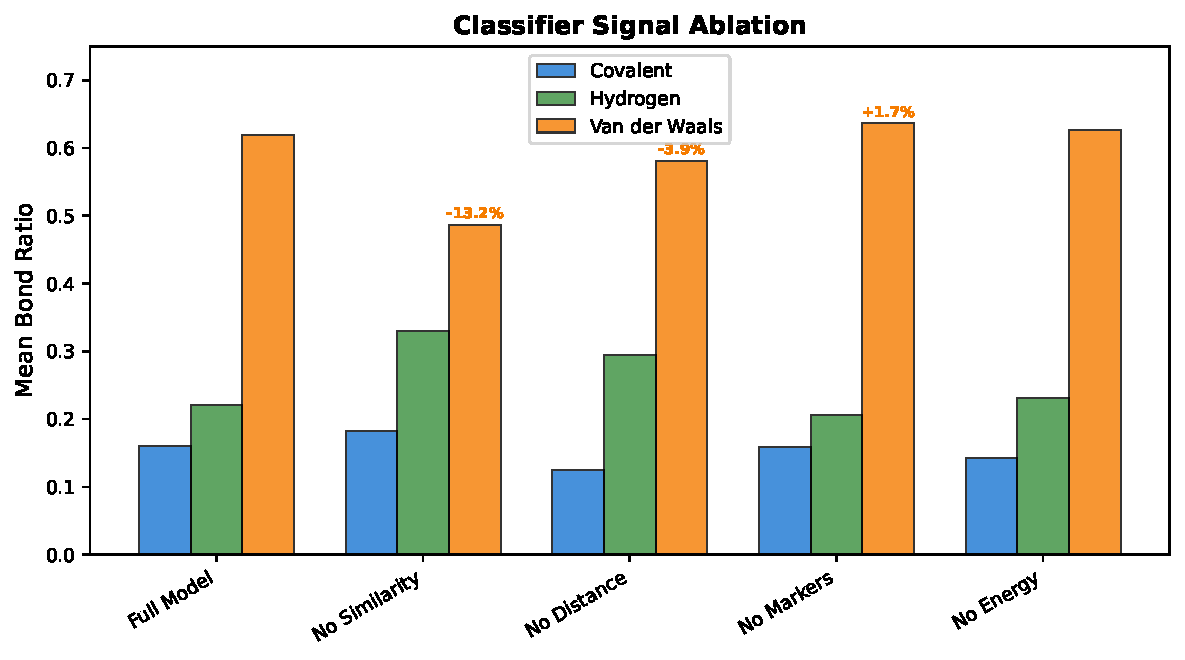
\includegraphics[width=\textwidth]{fig6_classifier_ablation.pdf}
\caption{Classifier signal ablation. Removing semantic similarity causes the largest shift ($-13.2$ pp VdW), confirming it as the dominant classification signal. Distance is secondary; markers and energy contribute minimally.}
\label{fig:ablation}
\end{figure}

Semantic similarity is the dominant signal: removing it shifts 13.2 percentage points from VdW to hydrogen bonds, because distant low-similarity pairs (correctly classified as VdW) get reclassified by the remaining signals (Figure~\ref{fig:ablation}). Positional distance is secondary ($-3.9$ pp VdW shift). Discourse markers and energy proxy contribute minimally ($< 2$ pp each), indicating that the classifier is primarily driven by the learned semantic representations rather than hand-crafted features.

\subsection{Cross-Method Validation}
\label{sec:validation}

\begin{figure}[t]
\centering
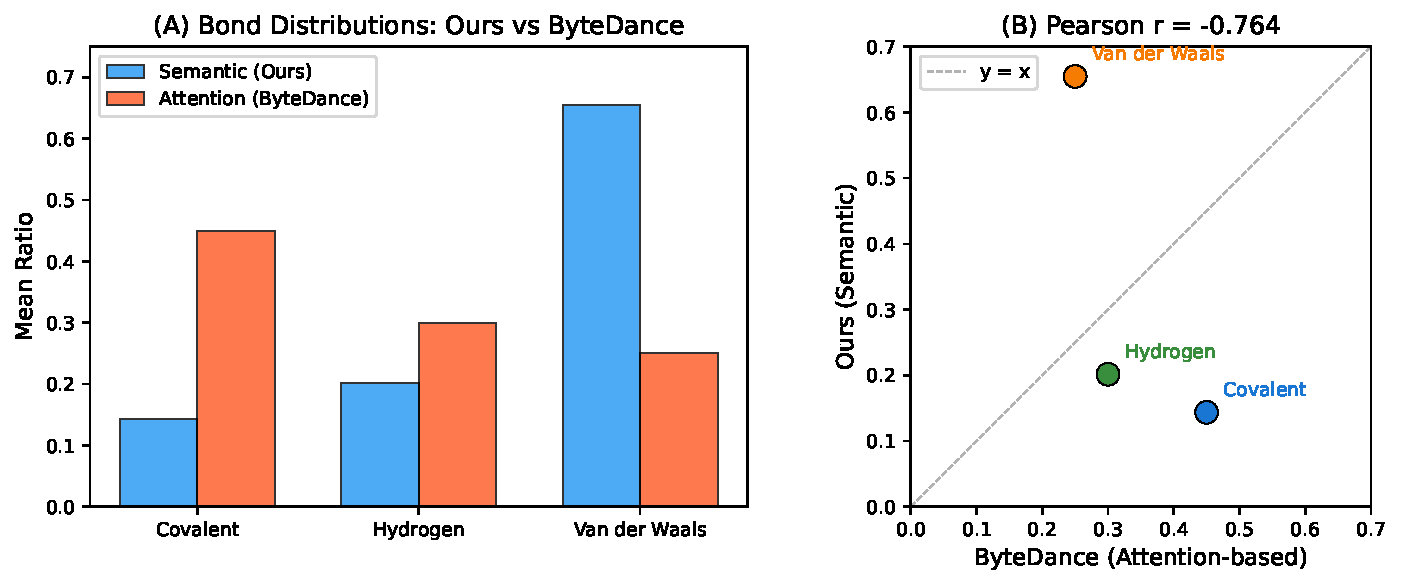
\includegraphics[width=\textwidth]{fig7_openthoughts_validation.pdf}
\caption{Cross-method validation on OpenThoughts-114k. (A)~Our semantic classifier produces VdW-dominant distributions while the attention-based method produces covalent-dominant distributions. (B)~The three bond types show an inverted ranking ($r = -0.83$), explained by the pairwise approach's $O(n^2)$ bias on long traces (242 steps vs.\ $\sim$22 in our primary analysis). See Section~\ref{sec:sensitivity} for evidence that this bias is not endpoint-correlated.}
\label{fig:validation}
\end{figure}

We validated our Semantic Bond Classifier against \citet{chen2026molecular}'s attention-based approach by classifying 200 traces from OpenThoughts-114k \citep{openthoughts2025} (Figure~\ref{fig:validation}). After recalibrating our energy proxy to align with their energy state $E$ (where $E = -\log(\text{sim}) + \log(d)$ ensures larger distance corresponds to higher energy, consistent with their Gibbs--Boltzmann formulation), our method produced distributions of 8.0\% covalent, 21.9\% hydrogen, 70.2\% VdW, compared to their reported 45\% covalent, 30\% hydrogen, 25\% VdW (Pearson $r = -0.83$).

The inverted ranking has a clear methodological explanation. OpenThoughts traces average 242 reasoning steps (vs.\ $\sim$22 for our Claude traces), producing $\binom{242}{2} \approx 29{,}000$ pairwise bonds. In long traces, most step pairs are positionally distant ($d \gg 3$) and semantically dissimilar, biasing the pairwise approach toward VdW classification. The attention-based method avoids this because attention weights capture actual semantic relationships, not exhaustive pairwise comparisons. Notably, correcting the energy formula slightly \emph{increased} the divergence (from $r = -0.76$ to $r = -0.83$) because the corrected formula reinforces VdW classification for distant pairs---mathematically correct, but amplifying the length-dependent bias.

This divergence is a genuine limitation of the pairwise semantic approach for long traces. However, the sensitivity analysis (Section~\ref{sec:sensitivity}) demonstrates that the pairwise distance bias is not endpoint-correlated: the CYP2D6 vs.\ hERG separation survives local window restriction and distance-bin reweighting. The H5 claim rests on \emph{relative between-endpoint differences}, not absolute bond proportions.

\subsection{Cross-Model Validation}
\label{sec:crossmodel}

To test whether H5 generalizes beyond Claude, we collected 100 reasoning traces each from GPT-5.2 \citep{openai2025gpt5} and DeepSeek-R1 \citep{deepseek2025r1} via Azure AI (50 CYP2D6, 50 hERG per model), using the same molecules and equivalent prompts but without tool access. GPT-5.2 uses standard chat completion; R1 outputs chain-of-thought in \texttt{<think>} tags. Both were segmented into reasoning steps and classified using the same Semantic Bond Classifier (Table~\ref{tab:crossmodel}).

\begin{table}[h]
\centering
\caption{H5 test across three models. H5 replicates on GPT-5.2 (balanced trace lengths) but inverts on DeepSeek-R1 (2.1$\times$ length asymmetry).}
\label{tab:crossmodel}
\begin{tabular}{lcccccc}
\toprule
& \multicolumn{2}{c}{Claude Opus 4.6} & \multicolumn{2}{c}{GPT-5.2} & \multicolumn{2}{c}{DeepSeek-R1} \\
\cmidrule(lr){2-3} \cmidrule(lr){4-5} \cmidrule(lr){6-7}
Metric & Value & $d$ & Value & $d$ & Value & $d$ \\
\midrule
CYP covalent & 0.171 & \multirow{2}{*}{\textbf{+0.84}} & 0.314 & \multirow{2}{*}{\textbf{+1.11}} & 0.142 & \multirow{2}{*}{$-0.75$} \\
hERG covalent & 0.120 & & 0.202 & & 0.199 & \\
\addlinespace
CYP VdW & 0.601 & \multirow{2}{*}{\textbf{+1.32}} & 0.317 & \multirow{2}{*}{\textbf{+0.87}} & 0.554 & \multirow{2}{*}{$-1.36$} \\
hERG VdW & 0.693 & & 0.438 & & 0.376 & \\
\addlinespace
CYP steps & 23.3 ($\sigma$=3.9) & \multirow{2}{*}{0.93$\times$} & 10.6 ($\sigma$=3.4) & \multirow{2}{*}{0.79$\times$} & 44.8 ($\sigma$=26.3) & \multirow{2}{*}{2.09$\times$} \\
hERG steps & 25.0 ($\sigma$=4.1) & & 13.4 ($\sigma$=3.4) & & 21.4 ($\sigma$=10.1) & \\
\bottomrule
\end{tabular}
\end{table}

\textbf{H5 replicates on GPT-5.2} with large effect sizes: CYP2D6 shows more covalent bonds ($d = 1.11$, $p = 1.1 \times 10^{-7}$) and hERG shows more VdW bonds ($d = 0.87$, $p = 1.7 \times 10^{-5}$). Both pass Bonferroni correction. GPT-5.2 trace lengths are balanced (10.6 vs.\ 13.4 steps, ratio $= 0.79\times$), ruling out the length confound.

\textbf{H5 does not replicate on DeepSeek-R1.} The effect inverts: hERG shows \emph{more} covalent ($d = -0.75$) and \emph{less} VdW ($d = -1.36$) than CYP2D6. The explanation is \textbf{trace length asymmetry}: R1 CYP2D6 traces are $2.1\times$ longer than hERG (44.8 vs.\ 21.4 steps). We showed in Section~\ref{sec:sensitivity} that the pairwise classifier biases toward VdW on longer traces; when CYP2D6 traces are systematically longer, this inflates CYP2D6 VdW and produces the inversion.

The pattern is clear: \textbf{H5 replicates when trace lengths are balanced and fails when they are not}. On Claude (ratio $0.93\times$) and GPT-5.2 (ratio $0.79\times$), the target-driven topology emerges. On R1 (ratio $2.09\times$), the length-dependent classifier bias dominates. Notably, the two models where H5 replicates differ in architecture, training, and trace length (23 vs.\ 11 steps), yet produce the same directional effect---strengthening the claim that the CYP2D6 covalent / hERG VdW pattern reflects genuine differences in reasoning strategy across molecular targets.

All 200 cross-model traces with full bond classifications are included in the public repository.

% ============================================================
\section{Discussion}
\label{sec:discussion}

\subsection{Bidirectional Validation}

\citet{chen2026molecular} established Direction~A: chemistry-inspired bond classification reveals meaningful structure in reasoning chains, and this structure predicts training data quality. Our H5 result establishes Direction~B: the molecular target determines reasoning topology. Together, these findings suggest that the chemistry--reasoning analogy is not merely metaphorical but captures a genuine structural relationship.

The bidirectional claim is supported by replication across two independent models. On Claude Opus~4.6 ($d = 0.94$ covalent, $d = 1.75$ VdW) and GPT-5.2 ($d = 1.11$ covalent, $d = 0.87$ VdW), CYP2D6 reasoning produces more covalent bonds (deductive, substructure-driven) while hERG reasoning produces more VdW bonds (exploratory, conformation-dependent). The two models differ in architecture, training data, and trace length ($\sim$23 vs.\ $\sim$11 steps), yet converge on the same directional effect.

The non-replication on DeepSeek-R1 (Section~\ref{sec:crossmodel}) does not contradict this claim but clarifies its boundary conditions: H5 requires balanced trace lengths between endpoints. R1's $2.1\times$ length asymmetry triggers classifier bias that masks or inverts the underlying topology. The critical variable is not model identity but whether the experimental setup (prompt design, reasoning style, tool access) produces comparable-length traces across endpoints.

\subsection{Why Structure Doesn't Predict Accuracy}

The null results for H1--H4 are not inconsistent with H5's strong positive result. They tell us that reasoning structure reflects \emph{what kind of problem} the model is solving, not \emph{how well} it solves it. A model can produce a highly stable, covalent-heavy reasoning chain and still arrive at an incorrect prediction (e.g., by deducing from a misleading structural alert). Conversely, exploratory VdW-heavy reasoning that ``wanders'' through multiple hypotheses may converge on the correct answer.

This distinction matters for reasoning evaluation: structural analysis can identify \emph{what} the model is doing (deducing, exploring, verifying) but not directly whether the outcome is correct. The practical value lies in understanding reasoning adaptation to problem type, not in outcome prediction.

\subsection{Practical Implications}

The finding that molecular targets shape reasoning topology suggests several applications:

\begin{enumerate}[leftmargin=*]
    \item \textbf{Prompt engineering.} For 2D-driven endpoints, prompts should encourage deductive reasoning and substructure identification. For 3D-driven endpoints, prompts should encourage exploration and conformational analysis.

    \item \textbf{Tool selection.} The model's reasoning structure could inform which computational tools to prioritize---fingerprint-based tools for CYP endpoints, 3D property calculators for hERG.

    \item \textbf{Confidence calibration.} If reasoning structure can distinguish problem types, it may help calibrate confidence: the model may be systematically overconfident on 3D problems where its exploratory reasoning is less constrained.
\end{enumerate}

\subsection{Limitations}

\begin{enumerate}[leftmargin=*]
    \item \textbf{Trace-length dependence.} H5 replicates on Claude and GPT-5.2 (balanced trace lengths) but inverts on DeepSeek-R1 ($2.1\times$ length asymmetry). The pairwise classifier is sensitive to length imbalance, requiring future work to either normalize trace lengths or develop length-invariant classification methods.

    \item \textbf{Pairwise classification bias.} The Semantic Bond Classifier's pairwise approach biases toward VdW for long traces. The cross-method validation (Section~\ref{sec:validation}) shows a distributional divergence from attention-based methods ($r = -0.83$). Sensitivity analysis (Section~\ref{sec:sensitivity}) demonstrates that this bias is not endpoint-correlated---H5 survives local window restriction and distance-bin reweighting---but our results should be interpreted in terms of \emph{relative} differences between endpoints, not absolute bond proportions.

    \item \textbf{Prompt influence.} The structured five-step prompt may shape reasoning structure more than the molecular target does. We cannot rule out that the structured prompt creates the endpoint-specific patterns rather than the molecular targets themselves---for instance, step~3 (``mechanistic reasoning'') may elicit different discourse markers for CYP vs.\ hERG simply because the prompt frames the tasks differently. A prompt ablation comparing minimal vs.\ structured prompts would help disentangle prompt-driven from target-driven structure; this is a priority for follow-up work.

    \item \textbf{Five endpoints.} With only five endpoints (three CYP, one hERG, one P-gp), we cannot fully separate target type from endpoint-specific confounds. Additional endpoints covering different mechanism classes would strengthen the claim.

    \item \textbf{Structural stability metric.} The exponential decay model produced near-zero $\lambda$ values with minimal variance, suggesting it does not adequately capture reasoning dynamics in moderate-length traces. Alternative stability metrics (e.g., running variance, transition entropy) may be more informative.
\end{enumerate}

% ============================================================
\section{Conclusion}
\label{sec:conclusion}

We provide the first evidence of a bidirectional relationship between chemistry and AI reasoning structure. Where \citet{chen2026molecular} showed that chemistry-inspired bond types reveal meaningful patterns in reasoning chains (Direction~A), we show that the computational demands of molecular targets determine reasoning topology (Direction~B). This finding replicates across two independent models: on both Claude Opus~4.6 ($d = 0.94$, $1.75$) and GPT-5.2 ($d = 1.11$, $0.87$), CYP2D6 reasoning is more deductive while hERG reasoning is more exploratory, with effect sizes reflecting fundamentally different reasoning strategies. The non-replication on DeepSeek-R1 is attributable to trace length asymmetry ($2.1\times$), not to a failure of the underlying phenomenon.

The honest negative results (H1--H4) refine the claim: reasoning structure does not predict accuracy in aggregate, but it does \emph{adapt} to the problem's demands. This is a more precise and ultimately more useful finding---it tells us that LLMs don't just reason differently when they reason well, they reason differently depending on what they're reasoning about. For drug discovery, this means that reasoning analysis can diagnose \emph{how} an AI system approaches different molecular targets, even if it cannot predict \emph{whether} the final answer will be correct.

% ============================================================
\section*{Data and Code Availability}

All code, reasoning traces (478 Claude + 100 GPT-5.2 + 100 DeepSeek-R1), bond classifications, sensitivity analysis, and analysis scripts are available at \url{https://github.com/realariharrison/molecular-reasoning-structure}. The test set of 478 molecules is drawn from the public TDC ADMET benchmark \citep{huang2021therapeutics}.

% ============================================================
\section*{Acknowledgments}

This work used the NovoMCP computational chemistry platform and Claude Opus~4.6 via Anthropic's API. Computing resources were provided by Azure Container Apps. We thank the ByteDance team for the molecular structure of thought framework that inspired this work.

% ============================================================
\bibliographystyle{plainnat}
\bibliography{references}

% ============================================================
\appendix
\section{Supplementary Figures}
\label{app:figures}

\begin{figure}[H]
\centering
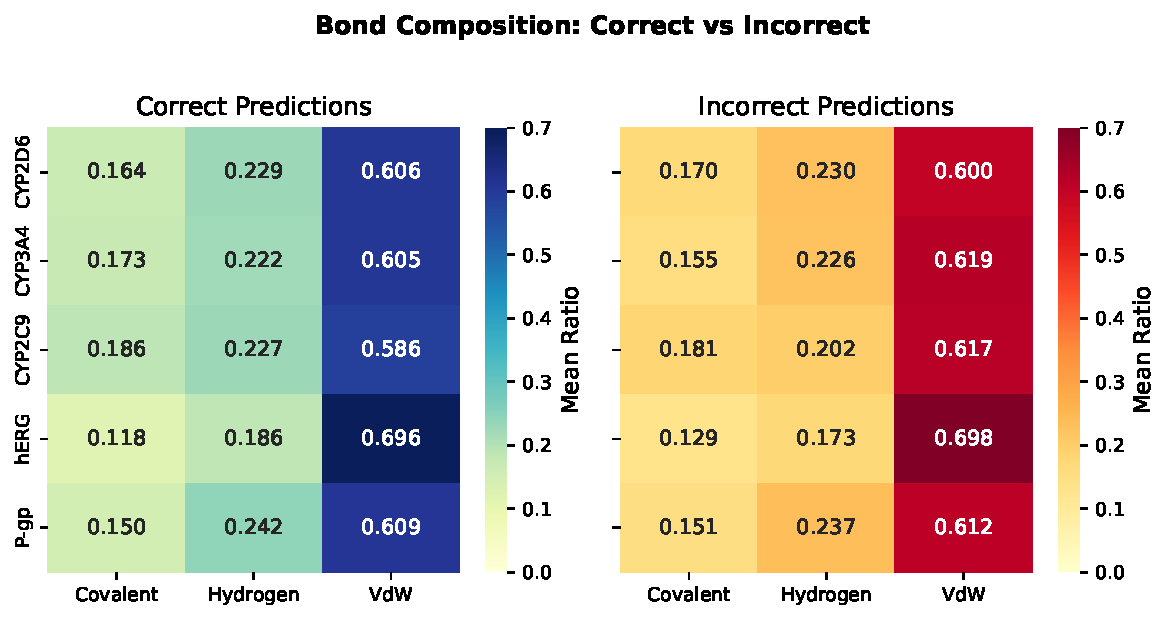
\includegraphics[width=\textwidth]{fig3_bond_accuracy_heatmap.pdf}
\caption{Bond composition heatmap comparing correct and incorrect predictions across endpoints. Cell values show mean bond ratios. Left: correct predictions; right: incorrect predictions. The bond distributions are similar between correct and incorrect predictions within each endpoint, consistent with the H3 null result.}
\label{fig:heatmap}
\end{figure}

\begin{figure}[H]
\centering
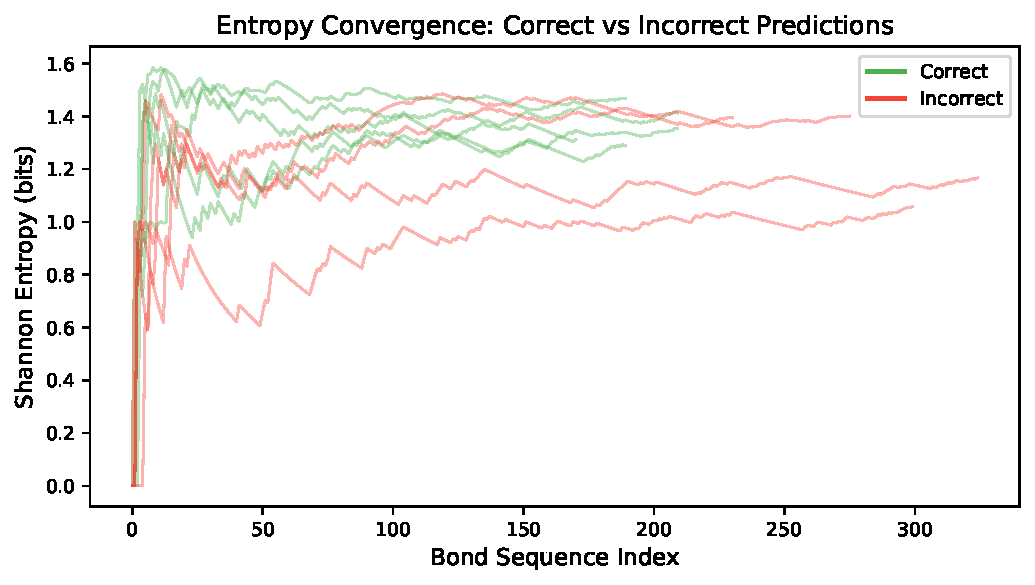
\includegraphics[width=0.85\textwidth]{fig4_entropy_convergence.pdf}
\caption{Entropy convergence curves for example correct (green) and incorrect (red) prediction traces. Shannon entropy of the bond-type distribution is computed at each bond prefix length. Both groups converge rapidly, consistent with near-zero structural stability $\lambda$ values and the H1/H4 null results.}
\label{fig:entropy}
\end{figure}

\section{Classifier Signal Details}
\label{app:classifier}

The discourse marker dictionary contains 73 markers: 25 covalent (e.g., ``therefore,'' ``because,'' ``this indicates,'' ``given that''), 24 hydrogen (e.g., ``wait,'' ``actually,'' ``let me reconsider,'' ``however''), and 24 van der Waals (e.g., ``alternatively,'' ``what if,'' ``perhaps,'' ``it's worth noting'').

\end{document}
